\section{Performance Evaluation}

To evaluate the performance of PQVRS, we carry out extensive real-world Internet experiments with real VR video display.

\subsection{System Overview}

PQVRS consists of 3 components: Viewpoint predicting module, JND computing module and bit-rate selection module, as shown in Fig. X.

(Figure)

In Viewpoint predicting module, we choose the method of ..., which can obtain ... accuracy.

Given the predicted viewpoint, JND computing module computes the scale factor of each tile.

After finishing JND computing, bit-rate selection module chooses proper bit-rate for each tile based on algorithm 1 or algorithm 2.

\subsection{Evaluation Setup}

Fig. \ref{network} shows the network topology in the experiment, which consists of a client and a server.

\begin{figure}
  \centering
  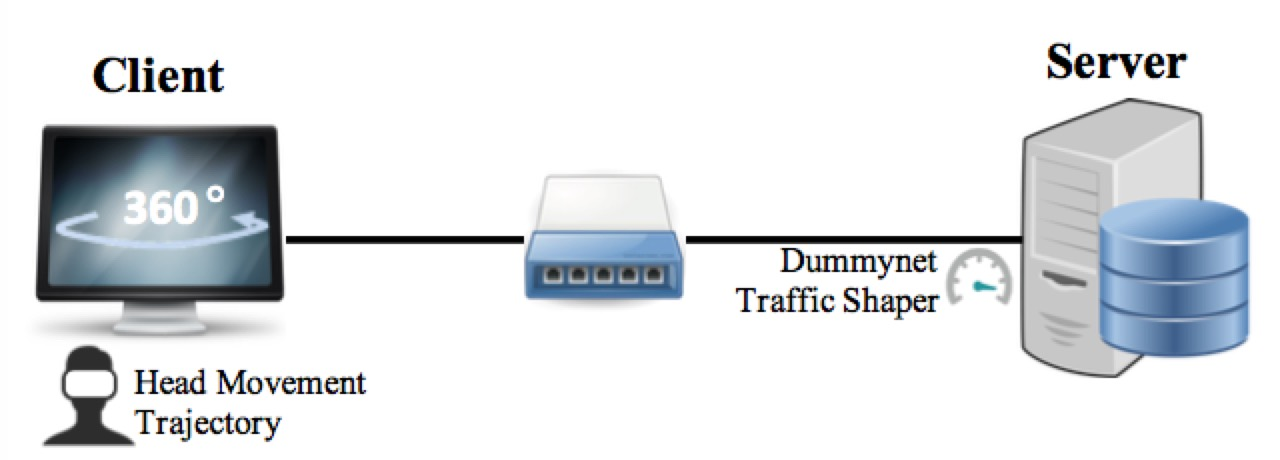
\includegraphics[width=3in]{images/network.jpg}
  \caption{Network topology.}
  \label{network}
  \end{figure}

In the experiments, we choose three videos in different types from the VR dataset. The information of these video is shown in Table 1. We set the duration of one video segment as 1 second. We adopt the 6 * 12 (rows * columns) tiling pattern for each video segment, thus the number of tiles is 72 (N = 72). To generate different quality videos, we use quantization parameter (QP) ranging from 22 to 42 in steps of five leading to five different bitrate versions. 

In our experiment, 5 different streaming methods are chosen to make comparison:

MONO: This approach is monolithic streaming. The naive way by streaming the entire 360-degree scene in constant QP without exploiting and optimizing the quality for the user’s viewport.

JND: This approach applies a traditional non-VR JND model (with consideration of content luminance, contrast and viewpoint heat map) to video coding. 

Viewpoint-driven streaming: Viewpoint prediction method is applied on client-side. For tiles in user's viewport, high quality is chosen. For other tiles, low quality is chosen.

PQVRS-: Viewpoint prediction method is applied on client-side. For tiles in user's viewport, a traditional non-VR JND model is applied to chose their quality. For other tiles, low quality is chosen.

PQVRS: Viewpoint prediction method is applied on client-side. For tiles in user's viewport, our proposed JND model is applied to chose their quality. For other tiles, low quality is chosen. This is the method presented in this paper.

\subsection{Performance Comparison}

\subsubsection{Quality-driven streaming}

In quality-driven streaming, perceived video quality is chosen by client. Adaptive Streaming logic needs to allocate bitrates of each tile each segment and minimize the bandwidth cost, while keeping user perceived quality unchanged.

Bandwidth comparison is shown in Fig. X.

Stalling comparison is shown in Fig. X.

In order to prove that different methods provide the same quality, a scoring system is designed based on real user.

\subsubsection{Streaming in constrained bandwidth}

In the real-world video streaming, VR video is streaming in a constraint bandwidth. Adaptive Streaming logic needs to adjust the video bit-rate based on current bandwidth estimation, while trying to maximizing the perceived quality.

Quality comparison is also made by our scoring system on real user. The result is shown in Fig. X.

\subsection{Insights from VR video display}

In order to clarify in which situation our proposed PQVRS has substantial improvement and in which situation its has marginal improvement, we choose one of the VR video display and plot the sequence diagram in Fig. \ref{sequence}. The displayed content is a skiing video. We highlight 5 frames to analyze the performance of 4 methods.

\begin{figure}
  \centering
  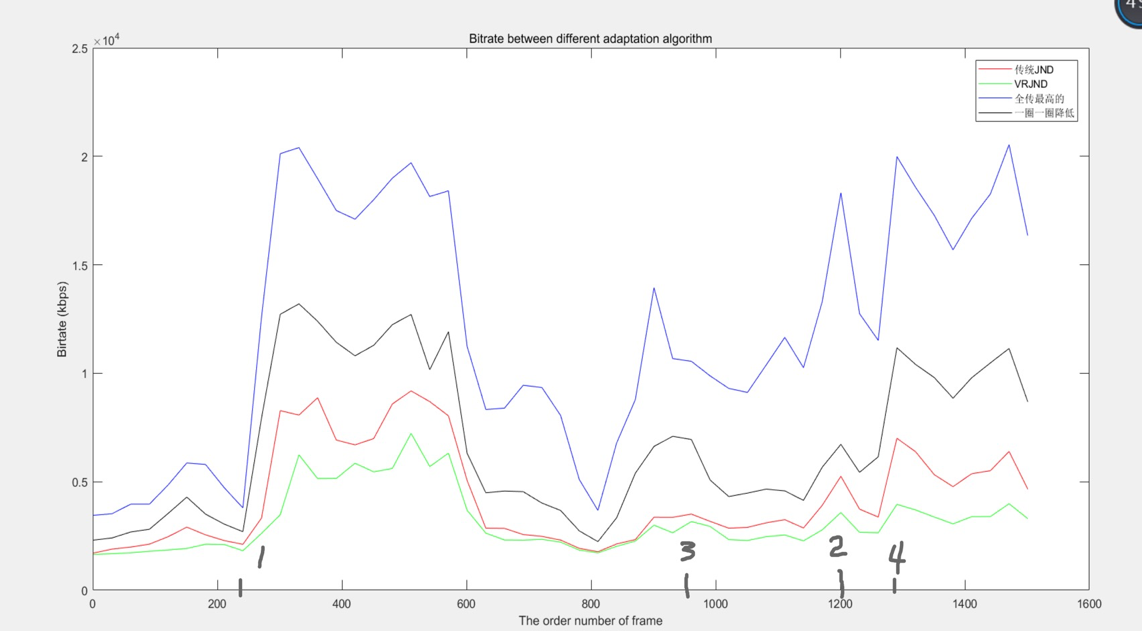
\includegraphics[width=3in]{images/sequence.png}
  \caption{Sequence diagram.}
  \label{sequence}
  \end{figure}

\begin{figure}
  \centering
  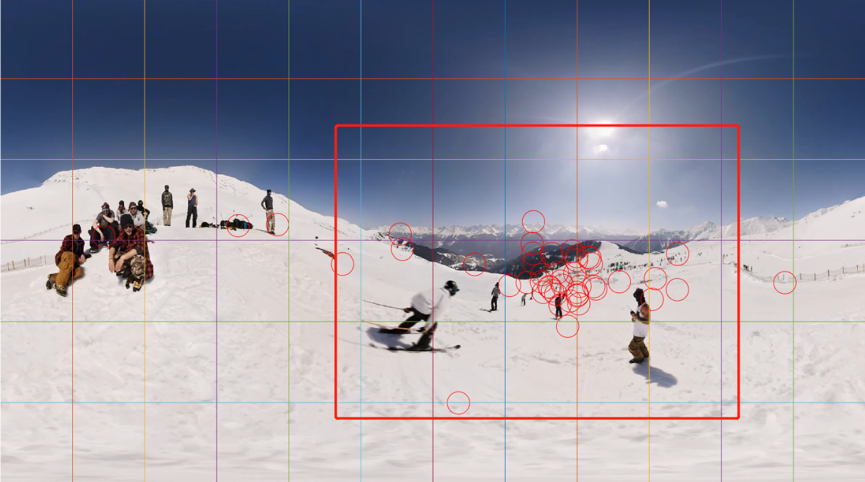
\includegraphics[width=3in]{images/case1.png}
  \caption{Frame A.}
  \label{referencename}
  \end{figure}
  
  \begin{figure}
  \centering
  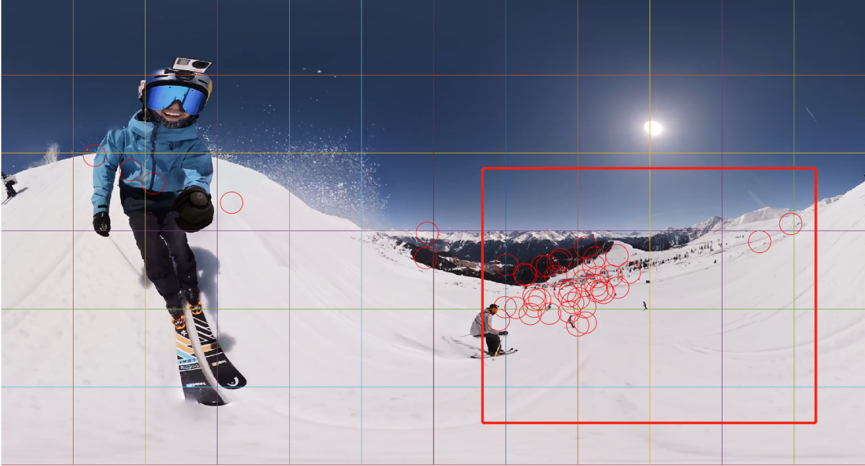
\includegraphics[width=3in]{images/case2.png}
  \caption{Frame B.}
  \label{referencename}
  \end{figure}
  
  \begin{figure}
  \centering
  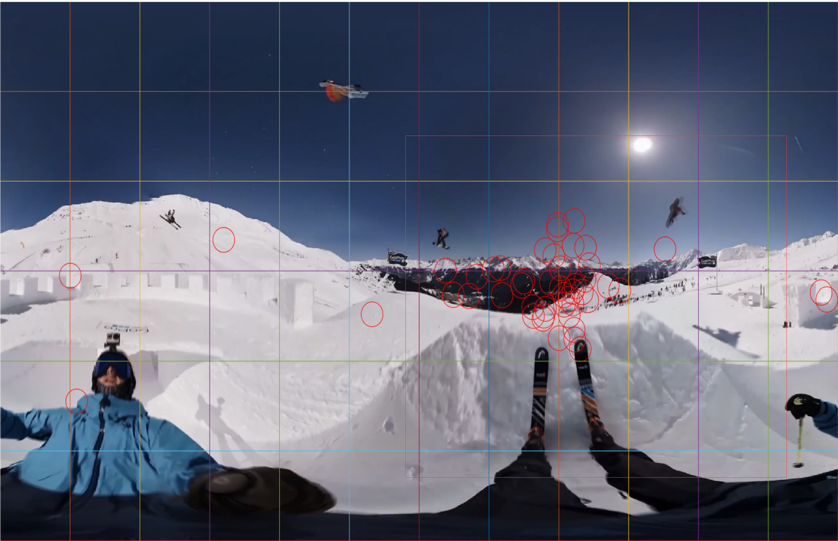
\includegraphics[width=3in]{images/case3.png}
  \caption{Frame C.}
  \label{referencename}
  \end{figure}
  
  \begin{figure}
  \centering
  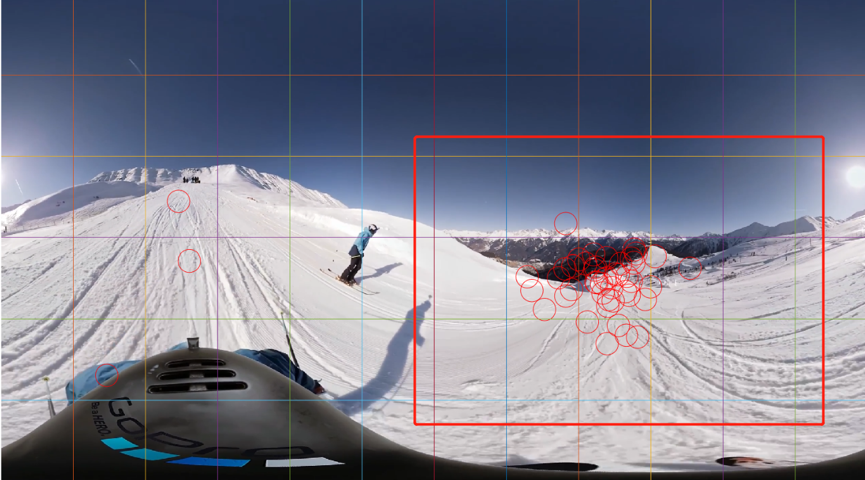
\includegraphics[width=3in]{images/case4.png}
  \caption{Frame D.}
  \label{referencename}
  \end{figure}

Frame A: 

Frame B: 

Frame C: 

Frame D: 

MONO performs well when ... .

Viewport driven Streaming

PQVRS-

PQVRS